\section{Experiment 10H-H: repair and validation of the single-model estimator}
\label{sec:experiment10hh}

\paragraph{Purpose and separation.}
Experiment 10H-G improved a normalized innovation objective, but its selected
fits exhausted their iteration budget. Source inspection also found an extra
covariance prediction after the prior Riccati solution and omission of the
covariance log-determinant. Experiment 10H-H repairs these issues before any
mixture or joint membership/model estimation. It reuses the five opened
development fleets 601--605, their measured records, the label-blind 20/10
training/held-out client split, and the three deterministic initializations.
This is a paired development repair, not a new blind confirmation. Seeds
611--620 remain sealed.

The estimator receives only yaw rate, lateral acceleration, applied steering,
steering command, and speed. True states, client parameters, class labels,
and exact client matrices remain behind the simulation boundary. A fixed
public nominal design supplies initial coordinates and bounds. The inherited
process-noise design and measurement covariance are frozen. Local trajectory
constant bias is estimated from the same quiet segment as in 10H-G.

\paragraph{Corrected covariance and objective.}
At each recorded speed, let $A(\theta),B(\theta)$ denote the structured
five-state model and let $C$ be its fixed measurement matrix. The filtering
Riccati equation is
\begin{equation}
 P=A\bigl(P-PC^\top(CPC^\top+R)^{-1}CP\bigr)A^\top+Q.
\end{equation}
Its solution is the \emph{prior} covariance. Consequently,
\begin{equation}
 S=CPC^\top+R,\qquad K=PC^\top S^{-1},
\end{equation}
without the additional $APA^\top+Q$ prediction used in 10H-G.
Every segment starts with zero posterior mean and stationary covariance.
With $\nu_t=y_t-C(A\hat x_{t-1}+Bu_t)$, the repaired objective is
\begin{equation}
 \mathcal L(\theta)=\frac{1}{3N_s}
 \sum_{t=1}^{N_s}
 \left[\nu_t^\top S^{-1}\nu_t+\log\det S-\log\det R\right].
 \label{eq:10hh-likelihood}
\end{equation}
The sensor-noise determinant is a parameter-independent reference. It makes
the reported objective positive and fixes the scale of its percentage changes,
but does not affect its minimizer. This is a stationary Gaussian
\emph{working likelihood}: one shared model is fitted to heterogeneous
vehicles, $Q$ is design tuning rather than identified process noise, and
quiet-segment bias-estimation uncertainty is not modeled explicitly.
It is not a correctly specified stochastic model of the entire fleet.
The fixed process-noise scale 0.01 was originally selected in 10H-A using
latent-state estimation errors. No 10H-H client truths are used to retune it,
but this inherited tuning means the complete covariance-selection pipeline
has not yet been demonstrated using measured outputs alone. The present
experiment validates the measured-array estimator interface with that design
setting held fixed. Subsequent covariance selection must use measured-output
validation if an entirely output-only training pipeline is claimed.

An independent predictive endpoint uses fixed sensor weights,
\begin{equation}
 \mathcal E_R(\theta)=\frac{1}{3N_s}
 \sum_t \nu_t^\top R^{-1}\nu_t.
\end{equation}
Improvement in this endpoint cannot be obtained merely by increasing $S$.
Both endpoints concern one-step measured-output prediction, not closed-loop
tracking or latent-state estimation.

\paragraph{Derivatives and optimization.}
Exact zero-order-hold matrix derivatives are evaluated with matrix-exponential
Fr\'echet derivatives. Put $M=I-KC$, $U=MP$, and $F=AM$. For log-coordinate
$\theta_j$, implicit Riccati differentiation gives
\begin{equation}
 P_j-FP_jF^\top=A_jUA^\top+AUA_j^\top.
\end{equation}
This discrete Lyapunov equation supplies $S_j$ and $K_j$. Forward
sensitivities propagate through the innovation and posterior-mean recursion.
The likelihood gradient includes all these derivatives and $\log\det S$.
Training-only diagonal information scaling preserves the original public box
bounds, from 0.35 to 3.0 times the nominal coordinates.

The frozen comparison includes a direct joint fit and a staged fit:
actuator rate first, relaxation rates second, and force/yaw coefficients third,
followed by full joint optimization. Both have a 300-iteration joint budget;
each restricted stage has an additional 80-iteration budget. This larger budget
is part of the repair, so numerical improvement is not attributed to gradients
alone. The full physical gate retains the declared restart, stationarity,
held-out, interior-bound, Hessian, and conditional-profile requirements.

\paragraph{Numerical and predictive results.}
Analytic gradients agree with central differences on every real development
fleet, with maximum norm-relative error $6.39\times10^{-8}$. Independent tests
also verify matrix derivatives, the Riccati fixed point, likelihood agreement
with a separate filter recursion, and constraint-gradient signs.

Every final optimizer call returns a success flag, but one joint-fit restart
on seed 605 terminates by small function reduction with projected gradient
0.551. Such a flag does not establish convergence. Its resulting coordinate
dispersion causes the joint numerical gate to fail. Staging repairs this:
all 15 staged restarts pass the projected-gradient check, their worst
coordinate CV is $1.71\times10^{-6}$, and their maximum objective spread is
$1.79\times10^{-10}$\%. Joint polishing takes 40--107 iterations, below its
300-iteration budget. No likelihood evaluation is invalid.

\begin{table}[htbp]
\centering
\caption{10H-H results on five opened development fleets, with three starts
per method and fleet. Prediction improvement is relative to the corrected
nominal model.}
\label{tab:10hh-results}
\begin{tabular}{lrr}
\toprule
Diagnostic & Joint & Staged\\
\midrule
Stationary final restarts & 14/15 & 15/15\\
Mean held-out $\mathcal L$ improvement & 18.57\% & 18.57\%\\
Minimum held-out $\mathcal L$ improvement & 12.24\% & 12.24\%\\
Mean held-out $\mathcal E_R$ improvement & 18.02\% & 18.02\%\\
Minimum held-out $\mathcal E_R$ improvement & 11.90\% & 11.90\%\\
Maximum restart parameter CV & 0.1365 & $1.71\times10^{-6}$\\
Maximum projected gradient & 0.551 & $1.25\times10^{-5}$\\
Fleets with an active bound & 5/5 & 5/5\\
Numerical repair gate & Fail & Pass\\
Full development gate & Fail & Fail\\
\bottomrule
\end{tabular}
\end{table}

The selected joint and staged solutions have effectively identical objectives
on every fleet. Mean fixed-weight prediction improvement is 18.02\%, with
fleet gains from 11.90\% to 25.38\%. Re-scoring the archived 10H-G vectors
with the corrected filter and objective gives 16.02\% mean likelihood and
15.71\% fixed-weight prediction improvement. These are valid paired
comparisons under the repaired scoring rule; the original 10H-G percentage
should not be compared directly with the new likelihood percentage.

\begin{figure}[htbp]
\centering
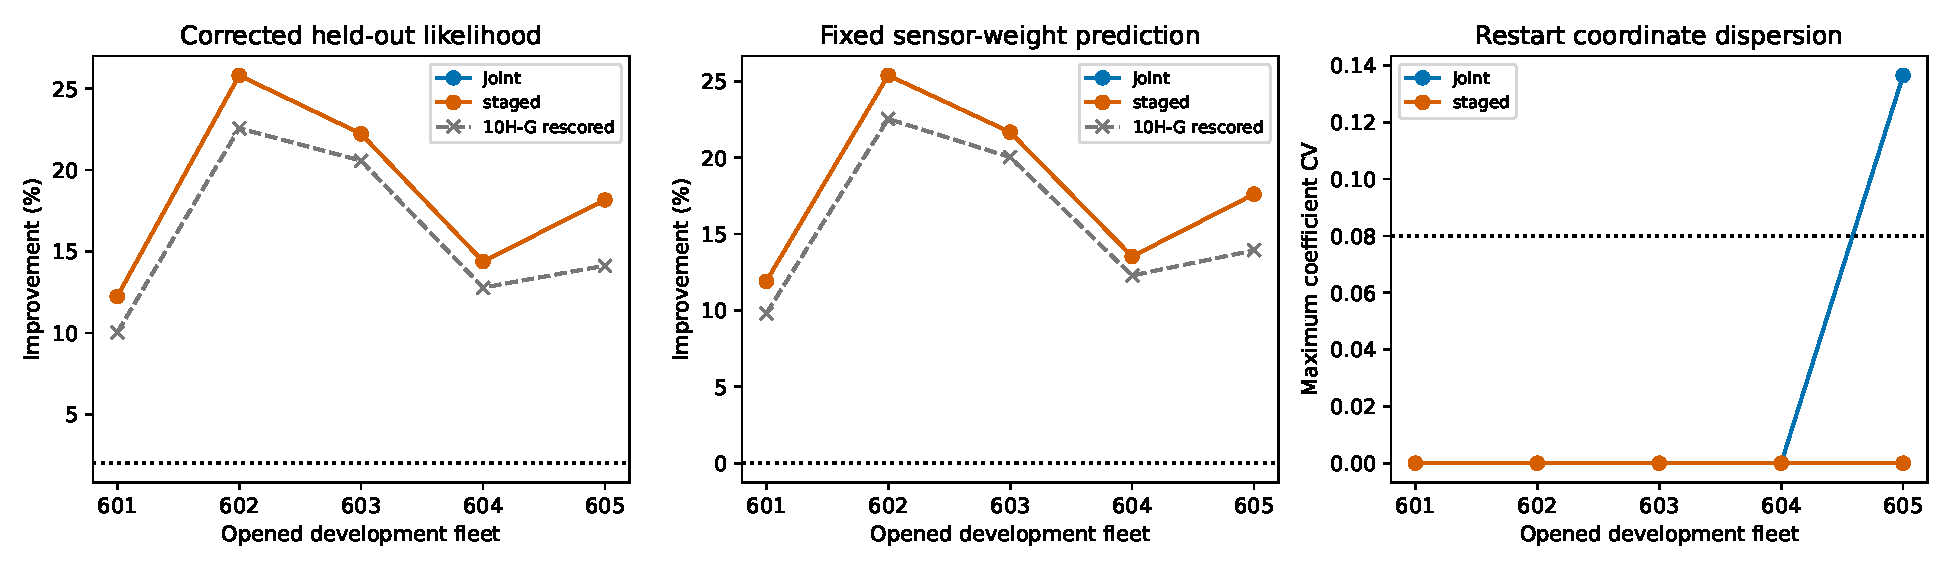
\includegraphics[width=0.98\linewidth]{../results/figures/experiment_10hh_single_model_repair.pdf}
\caption{Corrected held-out likelihood and fixed-weight prediction improvement,
plus restart dispersion. Archived 10H-G vectors are re-scored without refitting.}
\label{fig:10hh-repair}
\end{figure}

\paragraph{Boundary interpretation: a post-hoc diagnostic.}
The rear sideslip-to-force coefficient reaches its lower bound in all five
fleets. The corresponding front coefficient also reaches its upper bound in
three fleets. The full Hessian has a negative eigenvalue and clipped
conditional-profile edges can have zero increase, so the predeclared
interior-solution gate fails. These observations must not be misread as proof
that the staged optimizer has missed a constrained minimum.

A separate post-hoc audit leaves fitted vectors and all gates unchanged.
Every active-bound gradient has the appropriate Karush--Kuhn--Tucker sign.
The Hessian restricted to free coordinates is positive definite in every
selected fit, with minimum eigenvalue 0.0201. Thus the selected fits satisfy
the audited local constrained-minimum conditions. A zero outward profile
after clipping reflects the boundary, not an experimentally observed flat
direction.

\paragraph{Physical-model limitation.}
The same audit reveals that the nine effective coordinates do not all vary
independently in a physical bicycle model. Their definitions imply
\begin{equation}
 \frac{\varphi_{\mathrm{yaw,f}}\varphi_{\mathrm{front,\beta}}}
      {\varphi_{\mathrm{front,yaw}}}
 =
 \frac{\varphi_{\mathrm{yaw,r}}\varphi_{\mathrm{rear,\beta}}}
      {\varphi_{\mathrm{rear,yaw}}}
 =\frac{m}{I_z}.
 \label{eq:10hh-physical-coupling}
\end{equation}
Here $\varphi=\exp(\theta)$ denotes the positive effective coefficients.
The identity can be checked from fitted coefficients alone: actual mass,
inertia, geometry, and simulator truths are unnecessary. The two fitted
inertial-ratio expressions disagree by 29.52--79.42\%, normalized by their
mean. Consequently, an independently fitted nine-coordinate LPV model is
structurally anchored but need not correspond to one physical bicycle.
The development audit does not establish that this inconsistency causes the
bound activity; heterogeneous global pooling and the working covariance may
also contribute. These explanations require a controlled comparison.

\paragraph{Decision and next gate.}
The numerical repair succeeds with staged initialization: gradients are
validated, final fits are stationary and repeatable, and independently
weighted held-out prediction improves. The full physical-model gate remains
closed. The next experiment should enforce the exact common-inertial-ratio
identity through an eight-coordinate representation, using only measured
signals and public nominal bounds, and separate the effects of this physical
coupling from heterogeneous global pooling. It should retain the current
prediction and stationarity audits. Bounds should not be widened merely to
make the interior gate pass. Joint membership/model learning remains deferred
until this physical-model prerequisite is resolved.

The covariance convention also occurs in the historical 10H-A observer
helper. Its older observer/control results therefore need rechecking with
the corrected gain before those numerical results support the final
manuscript. This experiment repairs the identification interface and does
not re-evaluate those closed-loop studies.

\paragraph{Reproducibility.}
The protocol was fixed before fitting. The fit implementation and protocol
are archived in commit \texttt{112f35b}. Configuration,
estimator, runner, and numerical tests are stored in
\path{code/config/experiment_10hh.json},
\path{code/src/federated_lpv/innovation_likelihood.py},
\path{code/experiments/experiment_10hh_single_model_repair.py}, and
\path{code/tests/test_experiment_10hh.py}. Per-fleet and aggregate CSVs retain
restarts, phase outcomes, parameters, Hessian eigenvalues, conditional
profiles, gradient comparisons, data-split metadata, and measured-array
hashes. The post-hoc boundary/coupling audit has separate outputs and is
explicitly excluded from initial method selection and gate definitions.
